% !TEX TS-program = pdflatexmk
\documentclass[12pt]{article}

% Layout.
\usepackage[top=1in, bottom=0.75in, left=1in, right=1in, headheight=1in, headsep=6pt]{geometry}

% Fonts.
\usepackage{mathptmx}
\usepackage[scaled=0.86]{helvet}
\renewcommand{\emph}[1]{\textsf{\textbf{#1}}}
\newcommand{\ans}[1][1in]{\rule{#1}{.5pt}}

\usepackage[parfill]{parskip}

% Misc packages.
\usepackage{amsmath,amssymb,latexsym}
\usepackage{graphicx,hyperref}
\usepackage{array}
\usepackage{xcolor}
\usepackage{multicol,tikz}
\usepackage{tabularx,colortbl,booktabs,xparse}
\usepackage{enumitem}

\newcommand{\be}{\begin{enumerate}}
\newcommand{\ee}{\end{enumerate}}

% Rotation: \rot[<angle>][<width>]{<stuff>}
\NewDocumentCommand{\rot}{O{45} O{1em} m}{\makebox[#2][l]{\rotatebox{#1}{#3}}}%

\usepackage{fancyhdr}
\pagestyle{fancy} 
\lhead{\large\sf\textbf{MATH F113X: Eulerization}}
%\chead{\large\sf\textbf{lecture notes}}
%\rhead{\large\sf\textbf{Day 1}}

\begin{document}

\emph{Goals:} how to Eulerize a graph; why you would Eulerize a graph; how to put Dijkstra's algorithm together with Euler circuits (worksheet)

\begin{enumerate}
\item Given a graph, when can you find:
\be
\item An Euler circuit?
\vfill
\item An Euler path?
\vfill
\item Neither?
\vfill
\ee
\item Recall problem 5 from Worksheet 12:
\begin{quote}
\emph{Double} some of the edges so that every vertex is even degree. Using your additional edges, find an Euler circuit.
\end{quote}

%\begin{center}
%\begin{tikzpicture}[baseline=(current bounding box.center), scale=.4]
%\tikzstyle{every node}=[circle, draw, fill=black!0,
%                        inner sep=2pt, minimum width=10pt]
%\path (0,0) node (A) {A} ;
%\node (B)  at (-0,3) {B};
%\node (C) at (-3,0) {C} ;
%\node (E) at (-6,0) {E} ;
%\node (F) at (-6,3)  {F} ;
%\node (D) at (-3,3)  {D};
%\node (G) at (-9, 1.5) {G};
%\node (H) at (3,1.5) {H};
%\foreach \i/\j in {A/B,B/D,A/C, C/D, C/E,E/F,A/H,B/H, D/F,G/F, G/E}{\draw (\i) -- (\j);}
%\end{tikzpicture}
%\end{center}
%
%\bigskip
%
%
%\hrule

\quad\\
 %Below are several answers from the worksheet. What do you observe?\\
 %% Row 1
\begin{tabularx}{\textwidth}{XX}
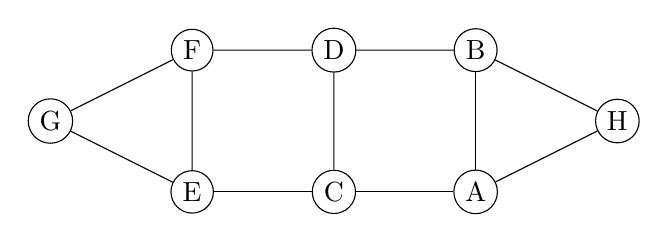
\begin{tikzpicture}[baseline=(current bounding box.center), scale=.6]
\tikzstyle{every node}=[circle, draw, fill=black!0,
                        inner sep=2pt, minimum width=10pt]
\path (0,0) node (A) {A} ;
\node (B)  at (-0,3) {B};
\node (C) at (-3,0) {C} ;
\node (E) at (-6,0) {E} ;
\node (F) at (-6,3)  {F} ;
\node (D) at (-3,3)  {D};
\node (G) at (-9, 1.5) {G};
\node (H) at (3,1.5) {H};
\foreach \i/\j in {A/B,B/D,A/C, C/D, C/E,E/F,A/H,B/H, D/F,G/F, G/E}{\draw (\i) -- (\j);}
\end{tikzpicture}
&
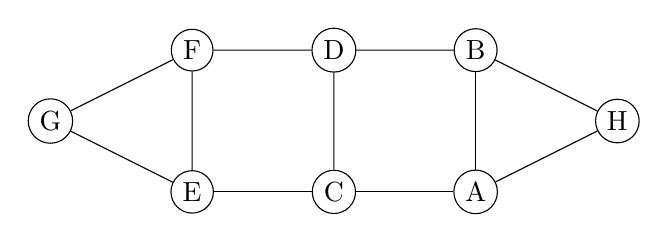
\begin{tikzpicture}[baseline=(current bounding box.center), scale=.6]
\tikzstyle{every node}=[circle, draw, fill=black!0,
                        inner sep=2pt, minimum width=10pt]
\path (0,0) node (A) {A} ;
\node (B)  at (-0,3) {B};
\node (C) at (-3,0) {C} ;
\node (E) at (-6,0) {E} ;
\node (F) at (-6,3)  {F} ;
\node (D) at (-3,3)  {D};
\node (G) at (-9, 1.5) {G};
\node (H) at (3,1.5) {H};
\foreach \i/\j in {A/B,B/D,A/C, C/D, C/E,E/F,A/H,B/H, D/F,G/F, G/E}{\draw (\i) -- (\j);}
\end{tikzpicture}
\end{tabularx}
\vfill
%%Row 2
\begin{tabularx}{\textwidth}{XX}
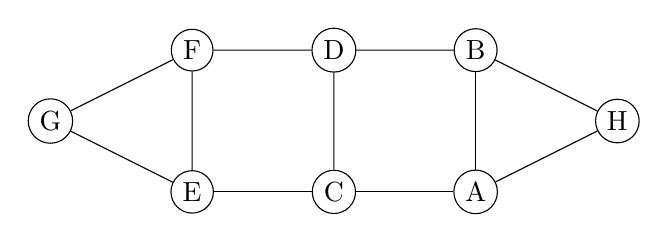
\begin{tikzpicture}[baseline=(current bounding box.center), scale=.6]
\tikzstyle{every node}=[circle, draw, fill=black!0,
                        inner sep=2pt, minimum width=10pt]
\path (0,0) node (A) {A} ;
\node (B)  at (-0,3) {B};
\node (C) at (-3,0) {C} ;
\node (E) at (-6,0) {E} ;
\node (F) at (-6,3)  {F} ;
\node (D) at (-3,3)  {D};
\node (G) at (-9, 1.5) {G};
\node (H) at (3,1.5) {H};
\foreach \i/\j in {A/B,B/D,A/C, C/D, C/E,E/F,A/H,B/H, D/F,G/F, G/E}{\draw (\i) -- (\j);}
\end{tikzpicture}
&
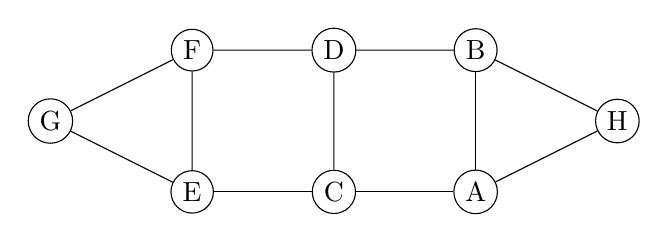
\begin{tikzpicture}[baseline=(current bounding box.center), scale=.6]
\tikzstyle{every node}=[circle, draw, fill=black!0,
                        inner sep=2pt, minimum width=10pt]
\path (0,0) node (A) {A} ;
\node (B)  at (-0,3) {B};
\node (C) at (-3,0) {C} ;
\node (E) at (-6,0) {E} ;
\node (F) at (-6,3)  {F} ;
\node (D) at (-3,3)  {D};
\node (G) at (-9, 1.5) {G};
\node (H) at (3,1.5) {H};
\foreach \i/\j in {A/B,B/D,A/C, C/D, C/E,E/F,A/H,B/H, D/F,G/F, G/E}{\draw (\i) -- (\j);}
\end{tikzpicture}
\end{tabularx}
\vfill
\item Some other examples\\
%Row 3
\begin{tabularx}{\textwidth}{XX}
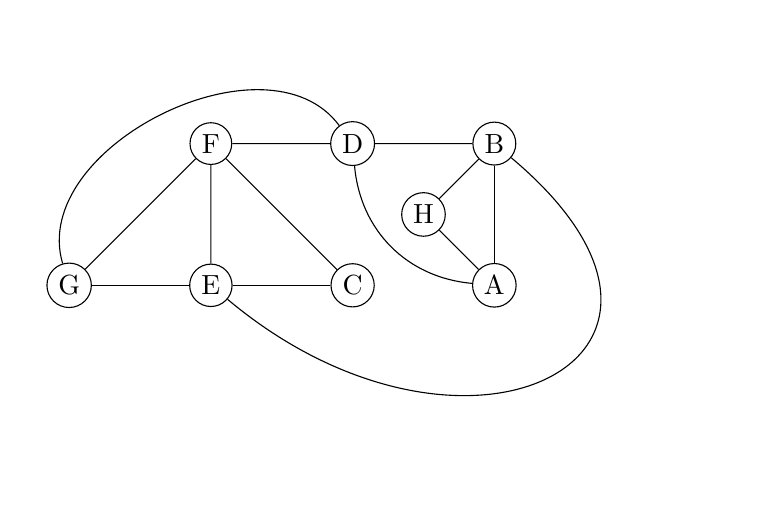
\begin{tikzpicture}[baseline=(current bounding box.center), scale=.6]
\tikzstyle{every node}=[circle, draw, fill=black!0,
                        inner sep=2pt, minimum width=10pt]
\path (0,0) node (A) {A} ;
\node (B)  at (-0,3) {B};
\node (C) at (-3,0) {C} ;
\node (E) at (-6,0) {E} ;
\node (F) at (-6,3)  {F} ;
\node (D) at (-3,3)  {D};
\node (G) at (-9, 0) {G};
\node (H) at (-1.5,1.5) {H};
% Unproblematic edges drawn straight
\draw (A) -- (B);
\draw (A) -- (H);
\draw (B) -- (H);
\draw (B) -- (D);
\draw (C) -- (E);
\draw (C) -- (F);
\draw (D) -- (F);
\draw (E) -- (F);
\draw (G) -- (E);
\draw (G) -- (F);

% A--D would cross B--C region; bend it above via the top
\draw (A) to[bend left=40] (D);

% E--B crosses C--D and A--C area; bend it upward above the grid
\draw (E) to[out=-40, in=-40, looseness=2.5] (B);

% G--D is very long and crosses E--D,F area; bend it above (northward arc)
\draw (G) to[bend left=80] (D);
\end{tikzpicture}
& \quad \quad \quad
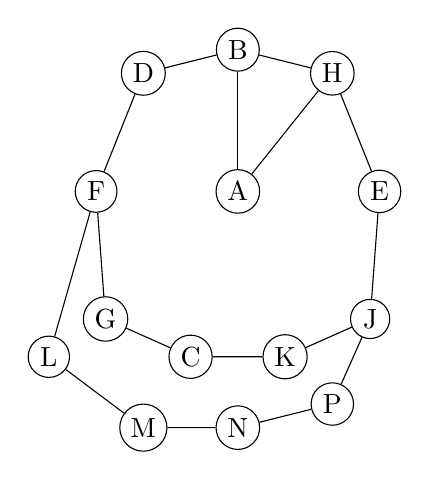
\begin{tikzpicture}[baseline=(current bounding box.center), scale=.6]
\tikzstyle{every node}=[circle, draw, fill=black!0,
                        inner sep=2pt, minimum width=10pt]
\path (0,0) node (A) {A} ;
\node (B)  at (0,3) {B};
\node (C) at (-1,-3.5) {C} ;
\node (E) at (3,0) {E} ;
\node (F) at (-3,0)  {F} ;
\node (D) at (-2,2.5)  {D};
\node (G) at (-2.8, -2.7) {G};
\node (H) at (2,2.5) {H};
\node (J) at (2.8,-2.7) {J};
\node (K) at (1,-3.5) {K};
\node (L) at (-4,-3.5) {L};
\node (M) at (-2, -5) {M};
\node (N) at (0,-5) {N};
\node (P) at (2,-4.5) {P};
\draw (F) -- (L) -- (M) -- (N) -- (P) -- (J);
\foreach \i/\j in {A/B,B/D,J/E, C/K,K/J,E/H,A/H,B/H, D/F,G/F, G/C}{\draw (\i) -- (\j);}
\end{tikzpicture}
\end{tabularx}
\vfill
\newpage
\item \textbf{Definition:} To \textbf{eulerize} a graph $G$ means\\

\vfill

\item \textbf{Definition:} An \textbf{optimal eulerization} means \\

\vfill

\item Under what conditions do you think it is \textit{easy} to obtain an optimal eulerization?

\vfill

\end{enumerate}
\end{document}